%%%%%%%%%%%%%%%%%%%%%%%%%%%%%%%%%%%%%%%%%
% Arsclassica Article
% LaTeX Template
% Version 1.1 (1/8/17)
%
% This template has been downloaded from:
% http://www.LaTeXTemplates.com
%
% Original author:
% Lorenzo Pantieri (http://www.lorenzopantieri.net) with extensive modifications by:
% Vel (vel@latextemplates.com)
%
% License:
% CC BY-NC-SA 3.0 (http://creativecommons.org/licenses/by-nc-sa/3.0/)
%
%%%%%%%%%%%%%%%%%%%%%%%%%%%%%%%%%%%%%%%%%

%----------------------------------------------------------------------------------------
%	PACKAGES AND OTHER DOCUMENT CONFIGURATIONS
%----------------------------------------------------------------------------------------

\documentclass[
10pt, % Main document font size
a4paper, % Paper type, use 'letterpaper' for US Letter paper
oneside, % One page layout (no page indentation)
%twoside, % Two page layout (page indentation for binding and different headers)
headinclude,footinclude, % Extra spacing for the header and footer
BCOR=5mm, % Binding correction
]{scrartcl}

%%%%%%%%%%%%%%%%%%%%%%%%%%%%%%%%%%%%%%%%%
% Arsclassica Article
% Structure Specification File
%
% This file has been downloaded from:
% http://www.LaTeXTemplates.com
%
% Original author:
% Lorenzo Pantieri (http://www.lorenzopantieri.net) with extensive modifications by:
% Vel (vel@latextemplates.com)
%
% License:
% CC BY-NC-SA 3.0 (http://creativecommons.org/licenses/by-nc-sa/3.0/)
%
%%%%%%%%%%%%%%%%%%%%%%%%%%%%%%%%%%%%%%%%%

%----------------------------------------------------------------------------------------
%	REQUIRED PACKAGES
%----------------------------------------------------------------------------------------
\usepackage[spanish, es-tabla]{babel} % Loads Spanish translations and fixes "Tabla"

\usepackage{silence}
% Silence specific package warnings
\WarningFilter{classicthesis}{Chapter sectioning command not present}
\WarningFilter{titlesec}{Non standard sectioning command}
\WarningFilter{remreset}{The remreset package is obsolete}
\WarningFilter{scrlayer-scrpage}{replacing deprecated}
\WarningFilter{hyperref}{Option}

\usepackage{silence}
% Silence specific package warnings
\WarningFilter{classicthesis}{Chapter sectioning command not present}
\WarningFilter{titlesec}{Non standard sectioning command}
\WarningFilter{remreset}{The remreset package is obsolete}
\WarningFilter{scrlayer-scrpage}{replacing deprecated}
\WarningFilter{hyperref}{Option}

\usepackage[
nochapters, % Turn off chapters since this is an article        
beramono, % Use the Bera Mono font for monospaced text (\texttt)
eulermath,% Use the Euler font for mathematics
pdfspacing, % Makes use of pdftex’ letter spacing capabilities via the microtype package
dottedtoc % Dotted lines leading to the page numbers in the table of contents
]{classicthesis} % The layout is based on the Classic Thesis style

\usepackage{arsclassica} % Modifies the Classic Thesis package

\usepackage[T1]{fontenc} % Use 8-bit encoding that has 256 glyphs

\usepackage[utf8]{inputenc} % Required for including letters with accents

\usepackage{graphicx} % Required for including images
\graphicspath{{Figures/}} % Set the default folder for images

\usepackage{enumitem} % Required for manipulating the whitespace between and within lists

\usepackage{amsmath,amssymb,amsthm} % For including math equations, theorems, symbols, etc

\usepackage{varioref} % More descriptive referencing

%----------------------------------------------------------------------------------------
%	THEOREM STYLES
%---------------------------------------------------------------------------------------

\theoremstyle{definition} 
\newtheorem{definition}{Definición}

\theoremstyle{plain} 
\newtheorem{theorem}{Teorema}

\theoremstyle{remark}

%----------------------------------------------------------------------------------------
%	HYPERLINKS
%---------------------------------------------------------------------------------------

\hypersetup{
%draft, % Uncomment to remove all links (useful for printing in black and white)
colorlinks=true, breaklinks=true, bookmarks=true,bookmarksnumbered,
urlcolor=webbrown, linkcolor=RoyalBlue, citecolor=webgreen, % Link colors
pdftitle={}, % PDF title
pdfauthor={\textcopyright}, % PDF Author
pdfsubject={}, % PDF Subject
pdfkeywords={}, % PDF Keywords
pdfcreator={pdfLaTeX}, % PDF Creator
pdfproducer={LaTeX with hyperref and ClassicThesis} % PDF producer
}


\graphicspath{{Figures/}}
\usepackage{float}    % Para usar el modificador [H]
\usepackage{subcaption} % Necesario para el entorno subfigure

\usepackage{tikz}
\usetikzlibrary{arrows.meta, babel}


%----------------------------------------------------------------------------------------
%	OBSERVACIONES
%---------------------------------------------------------------------------------------
\usepackage{tcolorbox}

% Definición del nuevo entorno para Observaciones
\newcounter{observacionnum} % Contador automático
\newenvironment{observacion}{%
    \stepcounter{observacionnum}%
    \begin{tcolorbox}[
        colback=white,          % Fondo blanco
        colframe=black,         % Borde negro
        arc=0mm,                % Esquinas completamente cuadradas
        boxrule=0.5pt,          % Grosor del borde exterior
        coltitle=black,         % Color del título
        fonttitle=\bfseries,    % Título en negrita
        title={Observación \arabic{observacionnum}}, % Texto del título
        attach title to upper,  % Junta el título con el contenido
        after title={\par\noindent\rule{\linewidth}{0.5pt}\par\medskip} % Línea debajo del título
    ]%
}{%
    \end{tcolorbox}%
}
 % Include the structure.tex file which specified the document structure and layout

\hyphenation{Fortran hy-phen-ation} % Specify custom hyphenation points in words with dashes where you would like hyphenation to occur, or alternatively, don't put any dashes in a word to stop hyphenation altogether

%----------------------------------------------------------------------------------------
%	TITLE AND AUTHOR(S)
%----------------------------------------------------------------------------------------

\title{\normalfont\spacedallcaps{Geometría epipolar}} % The article title

%\subtitle{Subtitle} % Uncomment to display a subtitle

\author{
    \spacedlowsmallcaps{Álvaro Acedo Blanco} \\ 
    \spacedlowsmallcaps{Daniel Czepiel Babiarz} \\ 
    \spacedlowsmallcaps{Séan Beltrán Amor}
}

\date{} % An optional date to appear under the author(s)

%----------------------------------------------------------------------------------------

\begin{document}

%----------------------------------------------------------------------------------------
%	HEADERS
%----------------------------------------------------------------------------------------

\renewcommand{\sectionmark}[1]{\markright{\spacedlowsmallcaps{#1}}} % The header for all pages (oneside) or for even pages (twoside)
%\renewcommand{\subsectionmark}[1]{\markright{\thesubsection~#1}} % Uncomment when using the twoside option - this modifies the header on odd pages
\lehead{\mbox{\llap{\small\thepage\kern1em\color{halfgray} \vline}\color{halfgray}\hspace{0.5em}\rightmark\hfil}} % The header style

\pagestyle{scrheadings} % Enable the headers specified in this block

%----------------------------------------------------------------------------------------
%	TABLE OF CONTENTS & LISTS OF FIGURES AND TABLES
%----------------------------------------------------------------------------------------

\maketitle % Print the title/author/date block

\setcounter{tocdepth}{2} % Set the depth of the table of contents to show sections and subsections only

\tableofcontents % Print the table of contents

\newpage % Start the article content on the second page, remove this if you have a longer abstract that goes onto the second page

%----------------------------------------------------------------------------------------
%	INTRODUCTION
%----------------------------------------------------------------------------------------

\section{Introducción}

Cuando tomamos una foto, proyectamos la imagen de un mundo tridimensional 
a uno bidimensional. Realizar esta proyección supone la pérdida de mucha 
información geométrica: los ángulos no se conservan, las distancias se deforman
y las rectas paralelas convergen a un punto.

Estas consecuencias nos recuerdan al paso de una geometría euclidiana a una 
proyectiva. Estando en la geometría euclidiana, las transformaciones preservan
distancias y ángulos. Cuando pasamos a la geometría afín, tenemos la posibilidad
de mover y deformar, perdiendo la conservación de ángulos y proporción de 
longitudes, pero manteniendo la diferencia entre puntos en el infinito y puntos
normales. Finalmente, en la geometría proyectiva no queremos esta diferencia,
provocando que las rectas paralelas se corten en el infinito.

De esta manera, veremos que la geometría proyectiva es el marco adecuado para
la creación y procesamiento de imágenes, pues la obtención de una no es más
que una proyección cónica y la intersección de esta con un plano. Nos apoyaremos
en la propiedad proyectiva de convertir rectas en rectas.


\subsection{¿Cómo manejamos que no haya rectas paralelas?}

El espacio proyectivo maneja esta cuestión añadiendo un hiperplano del infinito,
donde las rectas paralelas se cortan. Para trabajar con estos puntos en el plano
proyectivo $\mathbb{P}^2$, utilizamos coordenadas homogéneas $(x_1:x_2:x_3)$ donde un punto del 
infinito se representa con $x_3=0$, mientras que un punto finito tiene $x_3\neq0$ 
(normalmente se toma $x_3=1$). De esta manera, podemos tratar los puntos del infinito 
y los del espacio euclidiano sin necesidad de diferenciarlos, y convertir puntos del 
infinito en puntos normales y viceversa.

\subsection{¿Cómo analizamos los resultados en la geometría proyectiva?}

Conociendo todas las propiedades que no cumple la geometría proyectiva, podríamos
pensar que no podemos medir propiedades cercanas a las percepciones humanas. Pero
observamos que la geometría afín no es más que un caso particular de la geometría
proyectiva, y que la geometría euclidiana no es más que un caso particular de la 
geometría afín. 

Por lo tanto, podemos pasar de la proyectiva a la euclidiana mediante estos pasos::

\subsubsection{Caso de 2 dimensiones}

\paragraph{De proyectiva a afín}

El primero es pasar del proyectivo al afín. Esto lo conseguimos designando a
una recta como la recta del infinito, así, las rectas que se cortan en el infinito
son paralelas. Esto lo podríamos ver como definir la recta del horizonte.

\paragraph{De afín a euclidia}

El siguiente es pasar del afín al euclidiano. Primero tenemos que entender qué 
no cumplimos. En el plano afín deformamos las distancias, y como consecuencia,
no diferenciamos entre círculos y elipses, por ejemplo.

Observamos que las elipses se pueden cortar entre ellas hasta en 4 puntos, mientras
que las circunferencias como mucho se cortan en 2 puntos. La realidad es que
las circunferencias también se cortan en 4 puntos, solo que dos de estos puntos
están en el infinito. Así diferenciaremos las elipses de las circunferencias,
haciendo que estas últimas siempre corten en dos puntos especiales del infinito,
que llamaremos \textbf{puntos circulares}.

Haciendo el ejemplo con el producto escalar usual tenemos:

%TODO:Mirar si es cierto lo de que siempre debe tener solución
Sea el producto escalar usual $\langle (x,y),(x,y)\rangle = x^2+y^2$, 
que define la ecuación de una circunferencia, es decir, una cónica. 
Esta ecuación siempre debería tener una cónica como solución.

Pero hay un caso que parece que no cumple, este es cuando
$\|(x,y)\|=0$, que da $x^2+y^2=0$.

Sin embargo, si factorizamos, obtenemos:

\[
x^2+y^2 = (x+iy)(x-iy)=0,
\]
obteniendo los puntos circulares (en coordenadas homogéneas):
\[
I = [1:i:0], \qquad J = [1:-i:0].
\]

Por lo tanto, pasar del afín al euclidiano significa encontrar estos puntos circulares,
con los que conoceremos la métrica de la imagen.

\subsubsection{En 3 dimensiones}

En un espacio tridimensional se siguen los mismos pasos, solo que buscamos el
plano del infinito y, en vez de buscar los puntos circulares, buscamos la \textbf{cónica absoluta}
$\Omega_\infty$. 
Esta cónica, situada en el plano del infinito, codifica la estructura 
métrica del espacioeuclídeo.
Su imagen en una fotografía, denotada $\omega$, estña relacionada con los parámetros
intrinsecos de la cámara.

\subsubsection{Conclusión de la introducción}

Así, la geometría proyectiva puede verse como la más general.
La geometría afín se obtiene al distinguir una recta (o plano)
del infinito, mientras que la geometría euclídea se obtiene
añadiendo además una estructura métrica.

\subsection{Objetivo del trabajo}

Gracias a estos conocimientos de geometría proyectiva, podremos observar en el
trabajo que la relación entre dos imágenes está completamente codificada
en una matriz $3\times3$ llamada \textbf{matriz fundamental} $F$. 

A partir de F es posible reconstruir la escena hasta una
transformación proyectiva y obtener una estimación relativa de
la profundidad.

Si además conocemos la calibración (es decir, la imagen de la cónica absoluta), podemos 
trabajar con la \textbf{matriz esencial} $E$, que permite una reconstrucción métrica y, 
por tanto, un mapa de profundidad en unidades reales. 

%----------------------------------------------------------------------------------------
%	CÁMARA
%----------------------------------------------------------------------------------------

\section{Cámaras}

En esta sección vamos a hablar de las cámaras. La idea es trasladar la noción intuitiva que tenemos sobre una cámara a un objeto matemático formal con el que poder trabajar.

Si lo pensamos, lo que hace una cámara es proyectar un objeto del mundo tridimensional a una superficie bidimensional; es decir, se trata de una aplicación $c: \mathbb{R}^3 \rightarrow \mathbb{R}^2$. Con esta idea podemos dar una definición de lo que es una cámara:

\begin{definition}[Cámara]
    Una cámara es una transformación proyectiva desde el espacio proyectivo tridimensional $P\mathbb{R}^3$ al plano proyectivo bidimensional $P\mathbb{R}^2$.
\end{definition}

Para ver como modelamos está proyección vamos a ver primero un pequeño modelo físico.

\subsection{La cámara idealizada}

Una de las cámaras más simples que se pueden construir es la cámara estenopeica (\textit{pinhole camera}). Consiste en una caja sin lente con un pequeño orificio por el que pasa la luz y un material fotosensible que registra la imagen. El proceso físico de registro de la imagen se sale del ámbito de este trabajo; únicamente interesa la existencia de dicho mecanismo y la geometría con la que inciden los rayos de luz.

\begin{figure}[H]
    \centering
    \begin{subfigure}[b]{0.40\textwidth}
        \centering
        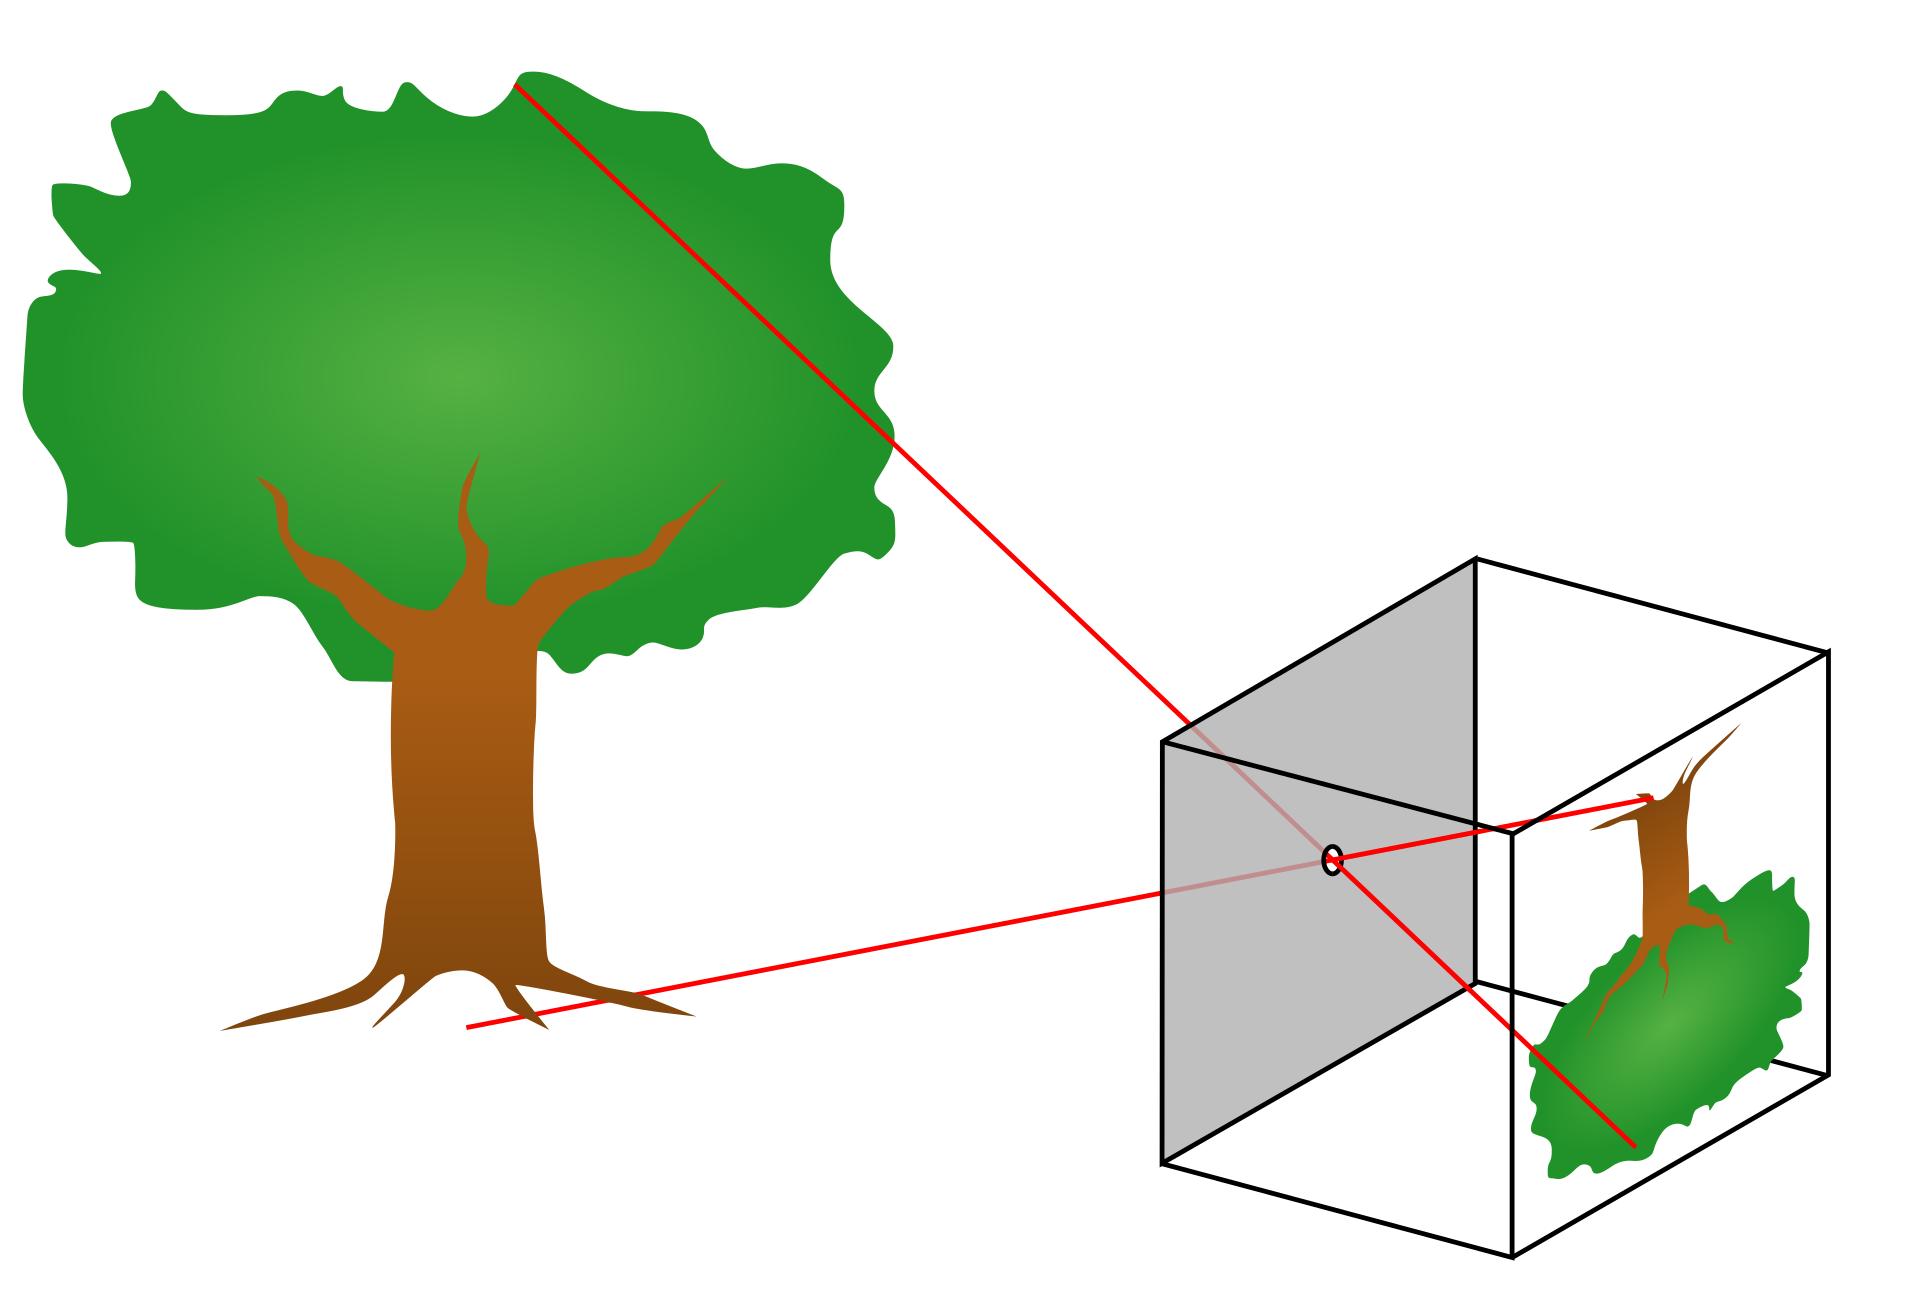
\includegraphics[width=\textwidth]{./Figures/Pinhole-camera.png}
        \caption{Modelo físico e intuitivo.}
        \label{fig:pinhole_fisica}
    \end{subfigure}
    \hfill % Genera espacio horizontal entre las dos imágenes
    \begin{subfigure}[b]{0.55\textwidth}
        \shorthandoff{>}\shorthandoff{<}
        \resizebox{\textwidth}{!}{
            \begin{tikzpicture}[scale=1.4, >=Stealth, every node/.style={font=\small}]
                % Centro de la cámara
                \coordinate (C) at (0,0);
                \filldraw (C) circle (2pt) node[below left] {$\mathbf{C}$};

                % Eje óptico / principal
                \draw[thick, dashed, ->] (C) -- (6,0) node[right] {Eje óptico};

                % Plano de la imagen (Perspectiva simulada mediante un plano inclinado)
                \draw[thick, fill=gray!10, fill opacity=0.6] (2.5,-1.5) -- (2.5,1.5) -- (3.3,2.0) -- (3.3,-1.0) -- cycle;
                \node[above] at (2.9,2.0) {Plano de la imagen};

                % Punto principal p (intersección del eje con el plano de la imagen)
                \coordinate (p) at (2.9, 0.25); 
                \filldraw (p) circle (1.5pt) node[below right] {$\mathbf{p}$};

                % Punto en el espacio X
                \coordinate (X) at (5.5, 1.8);
                \filldraw (X) circle (2pt) node[above right] {$\mathbf{X}$};

                % Rayo de luz proyectado desde C hasta X
                \draw[thick, color=blue!70!black] (C) -- (X);

                % Punto proyectado x (intersección exacta del rayo con el plano)
                \coordinate (x) at (2.92, 0.95); 
                \filldraw[red] (x) circle (1.5pt) node[above left, color=red] {$\mathbf{x}$};

                % Líneas auxiliares de proyección proyectadas sobre el eje
                \draw[gray, dotted] (X) -- (5.5,0);
                \draw[gray, dotted] (x) -- (2.92,0);

                % Acotación de la distancia focal f
                \draw[<->, gray] (0,-1.8) -- (2.5,-1.8) node[midway, below] {$f$};
                \draw[gray, dashed] (0,0) -- (0,-2.0);
                \draw[gray, dashed] (2.5,-1.5) -- (2.5,-2.0);
            \end{tikzpicture}
        }
        \caption{Modelo geométrico de la cámara estenopeica.}
        \label{fig:pinhole_tikz}
    \end{subfigure}
    \caption{Representación de la cámara estenopeica.}
    \label{pinhole_camera}
\end{figure}

Para modelar matemáticamente esta proyección, vamos a definir primero un par de conceptos.

\begin{definition}[Centro óptico]
    El centro óptico de la cámara se define formalmente como el núcleo (o espacio nulo) de la matriz de proyección $P$. Como veremos, su núcleo tiene dimensión 1,es decir, es un único punto $C \in \mathbb{P}^3$ tal que:
    \[
        P \cdot C = \mathbf{0}
    \]
\end{definition} 
\vspace{2ex}

\begin{observacion}
    Si nos fijamos en la Figura \ref{fig:pinhole_fisica}, podemos ver que el centro óptico es precisamente el pequeño agujero o estenopo que deja pasar la luz. Vamos a suponer que es suficientemente pequeño como para modelarlo como un único punto. Y efectivamente, al ser el núcleo de la aplicación, no esta definida la imagen de $C$.
\end{observacion}

\begin{definition}[Referencia cartesiana de la cámara y Eje principal]
    Al deshomogeneizar el espacio proyectivo, pasamos a trabajar en el espacio afín euclídeo tridimensional. Para formular el modelo, establecemos primero una referencia cartesiana ortonormal situando su origen en el centro óptico $\mathbf{C}$. Definimos el \textit{eje principal} (o eje óptico) haciéndolo coincidir con el eje $Z$ de esta referencia. El \textit{plano de la imagen} queda determinado de forma perpendicular a esta dirección $Z$. El punto de intersección entre el eje principal y el plano de la imagen se denomina \textit{punto principal}, denotado por $\mathbf{p}$.
\end{definition}
\vspace{2ex}

\begin{definition}[Distancia focal]
    Se define la \textit{distancia focal}, denotada por $f$, como la distancia euclídea entre el centro óptico $\mathbf{C}$ y el punto principal $\mathbf{p}$. Algebraicamente, $f$ actúa como el factor de escala intrínseco que relaciona el espacio tridimensional con el plano de proyección.
\end{definition} 
\vspace{2ex}

Con estos conceptos ya podemos calcular la matriz de proyección para esta configuración.

Fijamos nuestro sistema de referencia proyectivo situando el centro óptico en el origen, $\mathbf{C} = (0,0,0,1)^T$, y alineamos el eje óptico con el eje $Z$. Tal y como se estableció, el plano de la imagen se ubica en $Z = f$.

Dado un punto tridimensional en coordenadas homogéneas $\mathbf{X} = (X, Y, Z, 1)^T$, su proyección sobre el plano de la imagen resulta en un punto bidimensional. Si temporalmente deshomogeneizamos para observar el espacio afín, la semejanza de triángulos dicta que las coordenadas de la proyección son:
\[
    x = f \frac{X}{Z}, \quad y = f \frac{Y}{Z}
\]

\begin{figure}[H]
    \centering
    \begin{tikzpicture}[scale=1.2, >=Stealth, every node/.style={font=\small}]
        % Centro de la cámara
        \coordinate (C) at (0,0);

        % Eje óptico (Z)
        \draw[thick, dashed, ->] (0,0) -- (7,0) node[right] {Eje $Z$ (Profundidad)};
        \filldraw (C) circle (2pt) node[below left] {$\mathbf{C}$};

        % Plano de la imagen (Z = f)
        \def\f{2.5}
        \draw[thick, blue!80!black] (\f, -1.5) -- (\f, 3.5) node[above] {Plano de la imagen};
        \coordinate (p) at (\f, 0);
        \filldraw (p) circle (1.5pt) node[below right] {$\mathbf{p}$};

        % Punto tridimensional X
        \def\Z{6}
        \def\X{2.8}
        \coordinate (P3D) at (\Z, \X);
        \filldraw (P3D) circle (2pt) node[above right] {$\mathbf{X} = (X, Y, Z)$};

        % Rayo de luz
        \draw[thick, color=orange!80!black] (C) -- (P3D);

        % Punto proyectado x
        \def\x{\f*\X/\Z} % Semejanza: x = f * X / Z
        \coordinate (P2D) at (\f, \x);
        \filldraw[red] (P2D) circle (1.5pt) node[above left, text=red] {$\mathbf{x} = (x, y, f)$};

        % Líneas de proyección hacia el eje Z para formar los triángulos
        \draw[dashed, gray] (P3D) -- (\Z, 0) coordinate (Z_base);
        \draw[dashed, gray] (P2D) -- (\f, 0);

        % Sombreado de los triángulos semejantes
        \fill[blue!10, opacity=0.5] (C) -- (p) -- (P2D) -- cycle;
        \fill[orange!10, opacity=0.4] (P2D) -- (p) -- (Z_base) -- (P3D) -- cycle;

        % Acotaciones de distancias
        \draw[<->] (0, -0.6) -- (\f, -0.6) node[midway, below] {$f$};
        \draw[<->] (0, -1.2) -- (\Z, -1.2) node[midway, below] {$Z$};

        % Acotaciones de alturas
        \draw[<->] (\Z+0.3, 0) -- (\Z+0.3, \X) node[midway, right] {$X$};
        \draw[<->] (\f-0.3, 0) -- (\f-0.3, \x) node[midway, left] {$x$};

    \end{tikzpicture}
    \caption{Corte bidimensional del modelo estenopeico.}
    \label{fig:semejanza_triangulos}
\end{figure}

Para expresar esta relación como una aplicación lineal continua en el espacio proyectivo, definimos el punto proyectado en $\mathbb{P}^2$ como $\mathbf{x} = (x, y, 1)^T$. Algebraicamente, la transformación se formula como:
\[
    \begin{pmatrix}
        x \\
        y \\
        1
    \end{pmatrix}
    \sim
    \begin{pmatrix}
        fX \\
        fY \\
        Z
    \end{pmatrix}
    =
    \begin{pmatrix}
        f & 0 & 0 & 0 \\
        0 & f & 0 & 0 \\
        0 & 0 & 1 & 0 
    \end{pmatrix}
    \begin{pmatrix}
        X \\
        Y \\
        Z \\
        1 
    \end{pmatrix}
\]

Fijado el sistema de referencia en el centro óptico, la matriz $P_0$ depende exclusivamente de un único parámetro. Por esta razón, la cámara estenopeica ideal queda matemáticamente determinada en su totalidad por su centro $c$ su distancia focal $f$.

Esto nos motiva a dar la siguiente definición:

\begin{definition}[Cámara ideal]
    Se define la cámara ideal como un par $(R, f)$, donde $R = (C, \mathcal{B})$ es una referencia cartesiana ortonormal (con origen $C \in \mathbb{R}^3$ y base ortonormal $\mathcal{B}$ del espacio $\mathbb{R}^3$), y $f \in \mathbb{R}^+$ es la distancia focal.
\end{definition}

\subsection{Generalización del modelo ideal}

Al formular el modelo de la cámara ideal hemos partido de ciertas simplificaciones que no tienen por qué cumplirse estrictamente en una cámara real física. A continuación, vamos a ir eliminando estas suposiciones en la medida de lo posible para construir un modelo de cámara más general y realista.

\subsubsection{Desplazamiento del punto principal}

En el modelo ideal, asumimos que el origen de coordenadas del plano de la imagen coincide exactamente con el punto principal $\mathbf{p}$. Sin embargo, en la práctica, el sistema de coordenadas de la imagen no tiene porque cumplirse y mucho modelos, tiene su origen en una esquina.

Para corregir esto, introducimos un desplazamiento o traslación en el plano de la imagen. Si denotamos las coordenadas del punto principal en el sistema de referencia de la imagen como $(p_x, p_y)^T$, la proyección geométrica de un punto espacial $(X, Y, Z)^T$ pasa a ser:
\[
    x = f \frac{X}{Z} + p_x, \quad y = f \frac{Y}{Z} + p_y
\]

Para expresar esta traslación de forma lineal mediante coordenadas homogéneas, modificamos la matriz de proyección de la siguiente manera:
\[
    \begin{pmatrix}
        x \\
        y \\
        1
    \end{pmatrix}
    =
    \begin{pmatrix}
        f & 0 & p_x & 0 \\
        0 & f & p_y & 0 \\
        0 & 0 & 1 & 0
    \end{pmatrix}
    \begin{pmatrix}
        X \\
        Y \\
        Z \\
        1
    \end{pmatrix}
\]

De este modo, podemos la matriz de proyección queda como:
\[
    P = \begin{pmatrix} f & 0 & p_x & 0 \\ 0 & f & p_y & 0 \\ 0 & 0 & 1 & 0 \end{pmatrix}
\]

\subsubsection{Posición y orientación}

Hasta ahora se había asumido que la referencia cartesiana de la cámara coincidía con la referencia global del espacio tridimensional. Sin embargo, al modelar una escena general, y especialmente al tratar con varias cámaras simultáneamente, los puntos del espacio se expresan respecto a una referencia cartesiana global.

Dado que tanto la referencia del mundo como la de la cámara se exigen ortonormales, la transformación entre ambas consiste exclusivamente en una isometría del espacio euclídeo, es decir, una rotación y una traslación.

Geométricamente, para transformar un punto $\mathbf{X}_{\text{mundo}}$ al sistema local de la cámara, primero calculamos el vector relativo desde el centro óptico al punto, es decir, $(\mathbf{X}_{\text{mundo}} - \mathbf{C})$. A continuación, rotamos este vector para alinear los ejes del mundo con los de la cámara multiplicando por una matriz de rotación $R \in SO(3)$. Esta matriz está determinada por los ángulos que forman los ejes de ambas referencias.

Podemos definir esta matriz de forma constructiva: si la orientación de la cámara viene dada por una base ortonormal cuyos vectores unitarios direccionales son $\mathbf{u}, \mathbf{v}, \mathbf{w}$ expresados en las coordenadas del mundo, las filas de la matriz de rotación $R$ están formadas exactamente por estos vectores transpuestos:
\[
    R = \begin{pmatrix} \mathbf{u}^T \mathbf{v}^T \mathbf{w}^T \end{pmatrix}
\]

La expresión afín del cambio de coordenadas en el espacio tridimensional es:
\[
    \mathbf{X}_{\text{cam}} = R (\mathbf{X}_{\text{mundo}} - \mathbf{C}) = R \mathbf{X}_{\text{mundo}} - R \mathbf{C}
\]

Al pasar a coordenadas homogéneas, esta transformación se escribe de forma matricial utilizando notación por bloques. Siendo $R$ una matriz de $3 \times 3$, $-R\mathbf{C}$ un vector columna de $3 \times 1$ y $\mathbf{0}^T = (0,0,0)$ un vector fila, la matriz de transformación afín es de $4 \times 4$:
\[
    \begin{pmatrix}
        \mathbf{X}_{\text{cam}} \\
        1
    \end{pmatrix}
    =
    \begin{pmatrix}
        R_{3 \times 3} & (-R\mathbf{C})_{3 \times 1} \\
        \mathbf{0}^T_{1 \times 3} & 1
    \end{pmatrix}
    \begin{pmatrix}
        \mathbf{X}_{\text{mundo}} \\
        1
    \end{pmatrix}
\]

De esta deducción se extrae que el vector de traslación genérico de la cámara es $\mathbf{t} = -R\mathbf{C} \in \mathbb{R}^3$. Esta representación desvincula la rotación $R$ (orientación pura) de la traslación dependiente de la posición espacial del centro óptico $\mathbf{C}$.

Una vez el punto se encuentra en el sistema de referencia local de la cámara, se le puede aplicar directamente la matriz de calibración intrínseca para obtener su proyección en el plano de la imagen:
\[
    \mathbf{x} = K [I_{3 \times 3} \mid \mathbf{0}_{3 \times 1}] \begin{pmatrix} R & \mathbf{t} \\ \mathbf{0}^T & 1 \end{pmatrix} \begin{pmatrix} \mathbf{X}_{\text{mundo}} \\ 1 \end{pmatrix} = K [R \mid \mathbf{t}] \begin{pmatrix} \mathbf{X}_{\text{mundo}} \\ 1 \end{pmatrix}
\]

De este modo, la matriz de proyección general de la cámara $P$, de dimensiones $3 \times 4$, queda definida algebraicamente como el producto de sus parámetros intrínsecos y extrínsecos:
\[
    P = K [R \mid \mathbf{t}]
\]

\subsubsection{Píxeles no cuadrados y relación de aspecto}

Hasta ahora hemos considerado que ambos ejes de la imagen escalan de la misma forma geométrica. Sin embargo, en ciertos modelos de cámara, como puede ser aquellos equipados con sensores CCD, los elementos fotosensibles tienen forma rectangular en lugar de cuadrada. 

En consecuencia, el sistema de coordenadas de los píxeles pierde la condición de normalidad. Para modelar este escalado asimétrico, se introducen dos factores $k_x$ y $k_y$, que representan la densidad de píxeles por unidad de longitud en las direcciones horizontal y vertical. Esto desdobla la distancia focal en dos parámetros independientes, $f_x = f \cdot k_x$ y $f_y = f \cdot k_y$, modificando la matriz de calibración intrínseca $K$:
\[
    K = \begin{pmatrix}
        f_x & 0 & p_x \\
        0 & f_y & p_y \\
        0 & 0 & 1
    \end{pmatrix}
\]

\subsubsection{La cámara finita general}

Como hemos deducido en las secciones anteriores, la matriz de proyección general de la cámara se puede descomponer explícitamente aislando su centro óptico $\mathbf{C}$ de la siguiente manera:
\[
    P = K R [I_{3 \times 3} \mid -\mathbf{C}]
\]
Esta expresión agrupa los 11 grados de libertad del modelo en dos conjuntos fundamentales:
\begin{itemize}
    \item \textbf{Parámetros intrínsecos (matriz $K$):} Definen las propiedades internas y la geometría del sensor y son las distancias focales $f_x, f_y$ y el punto principal $(p_x, p_y)$.
    \item \textbf{Parámetros extrínsecos (matriz $R$ y centro $\mathbf{C}$):} Definen la posición espacial: centro de proyección $\mathbf{C}$ y la orientación: rotación ortogonal $R$, de la cámara respecto al sistema de coordenadas global del mundo.
\end{itemize}

Esta formulación asume que el centro óptico es un punto real y finito del espacio. Algebraicamente, esto nos lleva a la siguiente definición:

\begin{definition}[Cámara finita]
    Una cámara proyectiva finita es aquella cuya matriz de proyección $P$, de dimensiones $3 \times 4$, se descompone como $P = [M \mid \mathbf{p}_4]$, donde la submatriz izquierda $M$ de $3 \times 3$ es no singular ($\det(M) \neq 0$).
\end{definition}

\subsection{Cámaras en el infinito}

Como se ha visto en el desarrollo de la cámara finita se asume implícitamente que la submatriz izquierda $M$ de dimensiones $3 \times 3$ de la matriz de proyección $P = [M \mid \mathbf{p}_4]$ es no singular ($\det(M) \neq 0$). Esto garantiza que el centro óptico $\mathbf{C}$ se encuentra en un punto finito del espacio euclídeo.

Si se elimina esta restricción analítica y se permite que $\det(M) = 0$, el cálculo del núcleo de $P$ fuerza a que la última coordenada homogénea del centro óptico sea nula ($W=0$). Geométricamente, esto traslada el centro de proyección al infinito, lo que implica que los rayos de luz incidentes dejan de formar un cono convergente y pasan a ser paralelos. Este caso singular define los modelos de proyección paralela, los cuales se utilizan en visión artificial como una aproximación matemática robusta cuando el objeto observado está muy alejado respecto a su propio tamaño, anulando los efectos de la perspectiva dando mejores resultados que una cámara finita.

\begin{figure}[H]
    \centering
    % --- Subfigura 1: Cámara finita ---
    \begin{subfigure}[b]{0.48\textwidth}
        \centering
        \shorthandoff{>}\shorthandoff{<}
        \resizebox{\textwidth}{!}{
            \begin{tikzpicture}[scale=1.2, >=Stealth, every node/.style={font=\small}]
                % Centro óptico
                \coordinate (C) at (0,0);

                % Rayos proyectivos
                \draw[thick, orange!80!black, ->] (C) -- (5, 2.2);
                \draw[thick, orange!80!black, ->] (C) -- (5, 0);
                \draw[thick, orange!80!black, ->] (C) -- (5, -2.2);

                % Plano de la imagen
                \draw[thick, blue!80!black, fill=blue!10, fill opacity=0.7] (2, -2.2) -- (3, -1.7) -- (3, 2.2) -- (2, 1.7) -- cycle;
                \node[above] at (2.5, 2.0) {Plano de la imagen};

                % Puntos 3D
                \filldraw (5, 2.2) circle (2pt) node[right] {$\mathbf{X}_1$};
                \filldraw (5, 0) circle (2pt) node[right] {$\mathbf{X}_2$};
                \filldraw (5, -2.2) circle (2pt) node[right] {$\mathbf{X}_3$};

                % Puntos proyectados
                \filldraw[red] (2.5, 1.1) circle (1.5pt) node[above left, text=red] {$\mathbf{x}_1$};
                \filldraw[red] (2.5, 0) circle (1.5pt) node[above left, text=red] {$\mathbf{x}_2$};
                \filldraw[red] (2.5, -1.1) circle (1.5pt) node[below left, text=red] {$\mathbf{x}_3$};

                \filldraw (C) circle (2pt) node[left] {$\mathbf{C}$};
            \end{tikzpicture}
        }
        \caption{Cámara finita: Rayos convergentes.}
        \label{fig:rayos_finitos}
    \end{subfigure}
    \hfill
    % --- Subfigura 2: Cámara en el infinito ---
    \begin{subfigure}[b]{0.48\textwidth}
        \centering
        \shorthandoff{>}\shorthandoff{<}
        \resizebox{\textwidth}{!}{
            \begin{tikzpicture}[scale=1.2, >=Stealth, every node/.style={font=\small}]
                % Rayos proyectivos paralelos
                \draw[thick, orange!80!black, ->] (0, 1.5) -- (5, 1.5);
                \draw[thick, orange!80!black, ->] (0, 0) -- (5, 0);
                \draw[thick, orange!80!black, ->] (0, -1.5) -- (5, -1.5);

                % Rayos desde el infinito (discontinuos para dar sensación de lejanía)
                \draw[dashed, orange!80!black] (-1, 1.5) -- (0, 1.5);
                \draw[dashed, orange!80!black] (-1, 0) -- (0, 0);
                \draw[dashed, orange!80!black] (-1, -1.5) -- (0, -1.5);

                % Centro óptico en el infinito
                \node[left] at (-1, 0) {$\mathbf{C}_\infty$};

                % Plano de la imagen
                \draw[thick, blue!80!black, fill=blue!10, fill opacity=0.7] (2, -2.2) -- (3, -1.7) -- (3, 2.2) -- (2, 1.7) -- cycle;
                \node[above] at (2.5, 2.0) {Plano de la imagen};

                % Puntos 3D
                \filldraw (5, 1.5) circle (2pt) node[right] {$\mathbf{X}_1$};
                \filldraw (5, 0) circle (2pt) node[right] {$\mathbf{X}_2$};
                \filldraw (5, -1.5) circle (2pt) node[right] {$\mathbf{X}_3$};

                % Puntos proyectados
                \filldraw[red] (2.5, 1.5) circle (1.5pt) node[above left, text=red] {$\mathbf{x}_1$};
                \filldraw[red] (2.5, 0) circle (1.5pt) node[above left, text=red] {$\mathbf{x}_2$};
                \filldraw[red] (2.5, -1.5) circle (1.5pt) node[below left, text=red] {$\mathbf{x}_3$};
            \end{tikzpicture}
        }
        \caption{Cámara afín: Rayos paralelos.}
        \label{fig:rayos_infinitos}
    \end{subfigure}
    \caption{Comparación geométrica de los rayos de proyección entre los modelos de cámara.}
    \label{fig:comparacion_camaras}
\end{figure}

Aunque hacemos esta mención a las cámaras en el infinito por completitud analítica, para la siguiente sección de \textit{geometría epipolar} asumiremos de manera estricta el modelo de cámara finita general.

\newpage

%----------------------------------------------------------------------------------------
%	GEOMETRIA EPIPOLAR
%----------------------------------------------------------------------------------------
\section{Geometría epipolar}

La geometría epipolar es la geometría proyectiva intrínseca entre dos vistas. Depende exclusivamente de los parámetros internos de las cámaras y de su posición relativa, siendo completamente independiente de la estructura de la escena tridimensional.

Este concepto es fundamental en la Visión por Computador para el análisis geométrico de múltiples imágenes de una misma escena. Constituye la primera fase de la reconstrucción tridimensional, restringiendo y facilitando la búsqueda de correspondencias de píxeles entre distintas vistas.

\subsection{Fundamentos geométricos y elementos básicos}

Para modelar analíticamente esta relación, consideramos dos cámaras finitas descritas por sus matrices de proyección $P_1$ y $P_2$, que actúan como aplicaciones lineales continuas sobre el espacio proyectivo:
\[
    P_1, P_2: P\mathbb{R}^3 \longrightarrow P\mathbb{R}^2
\]

Sea $\mathbf{X} \in P\mathbb{R}^3$ un punto de la escena tridimensional cuyas proyecciones en los respectivos planos imagen son los puntos $\mathbf{x}_1 = P_1 \mathbf{X}$ y $\mathbf{x}_2 = P_2 \mathbf{X}$. 

\begin{figure}[H]
    \centering
    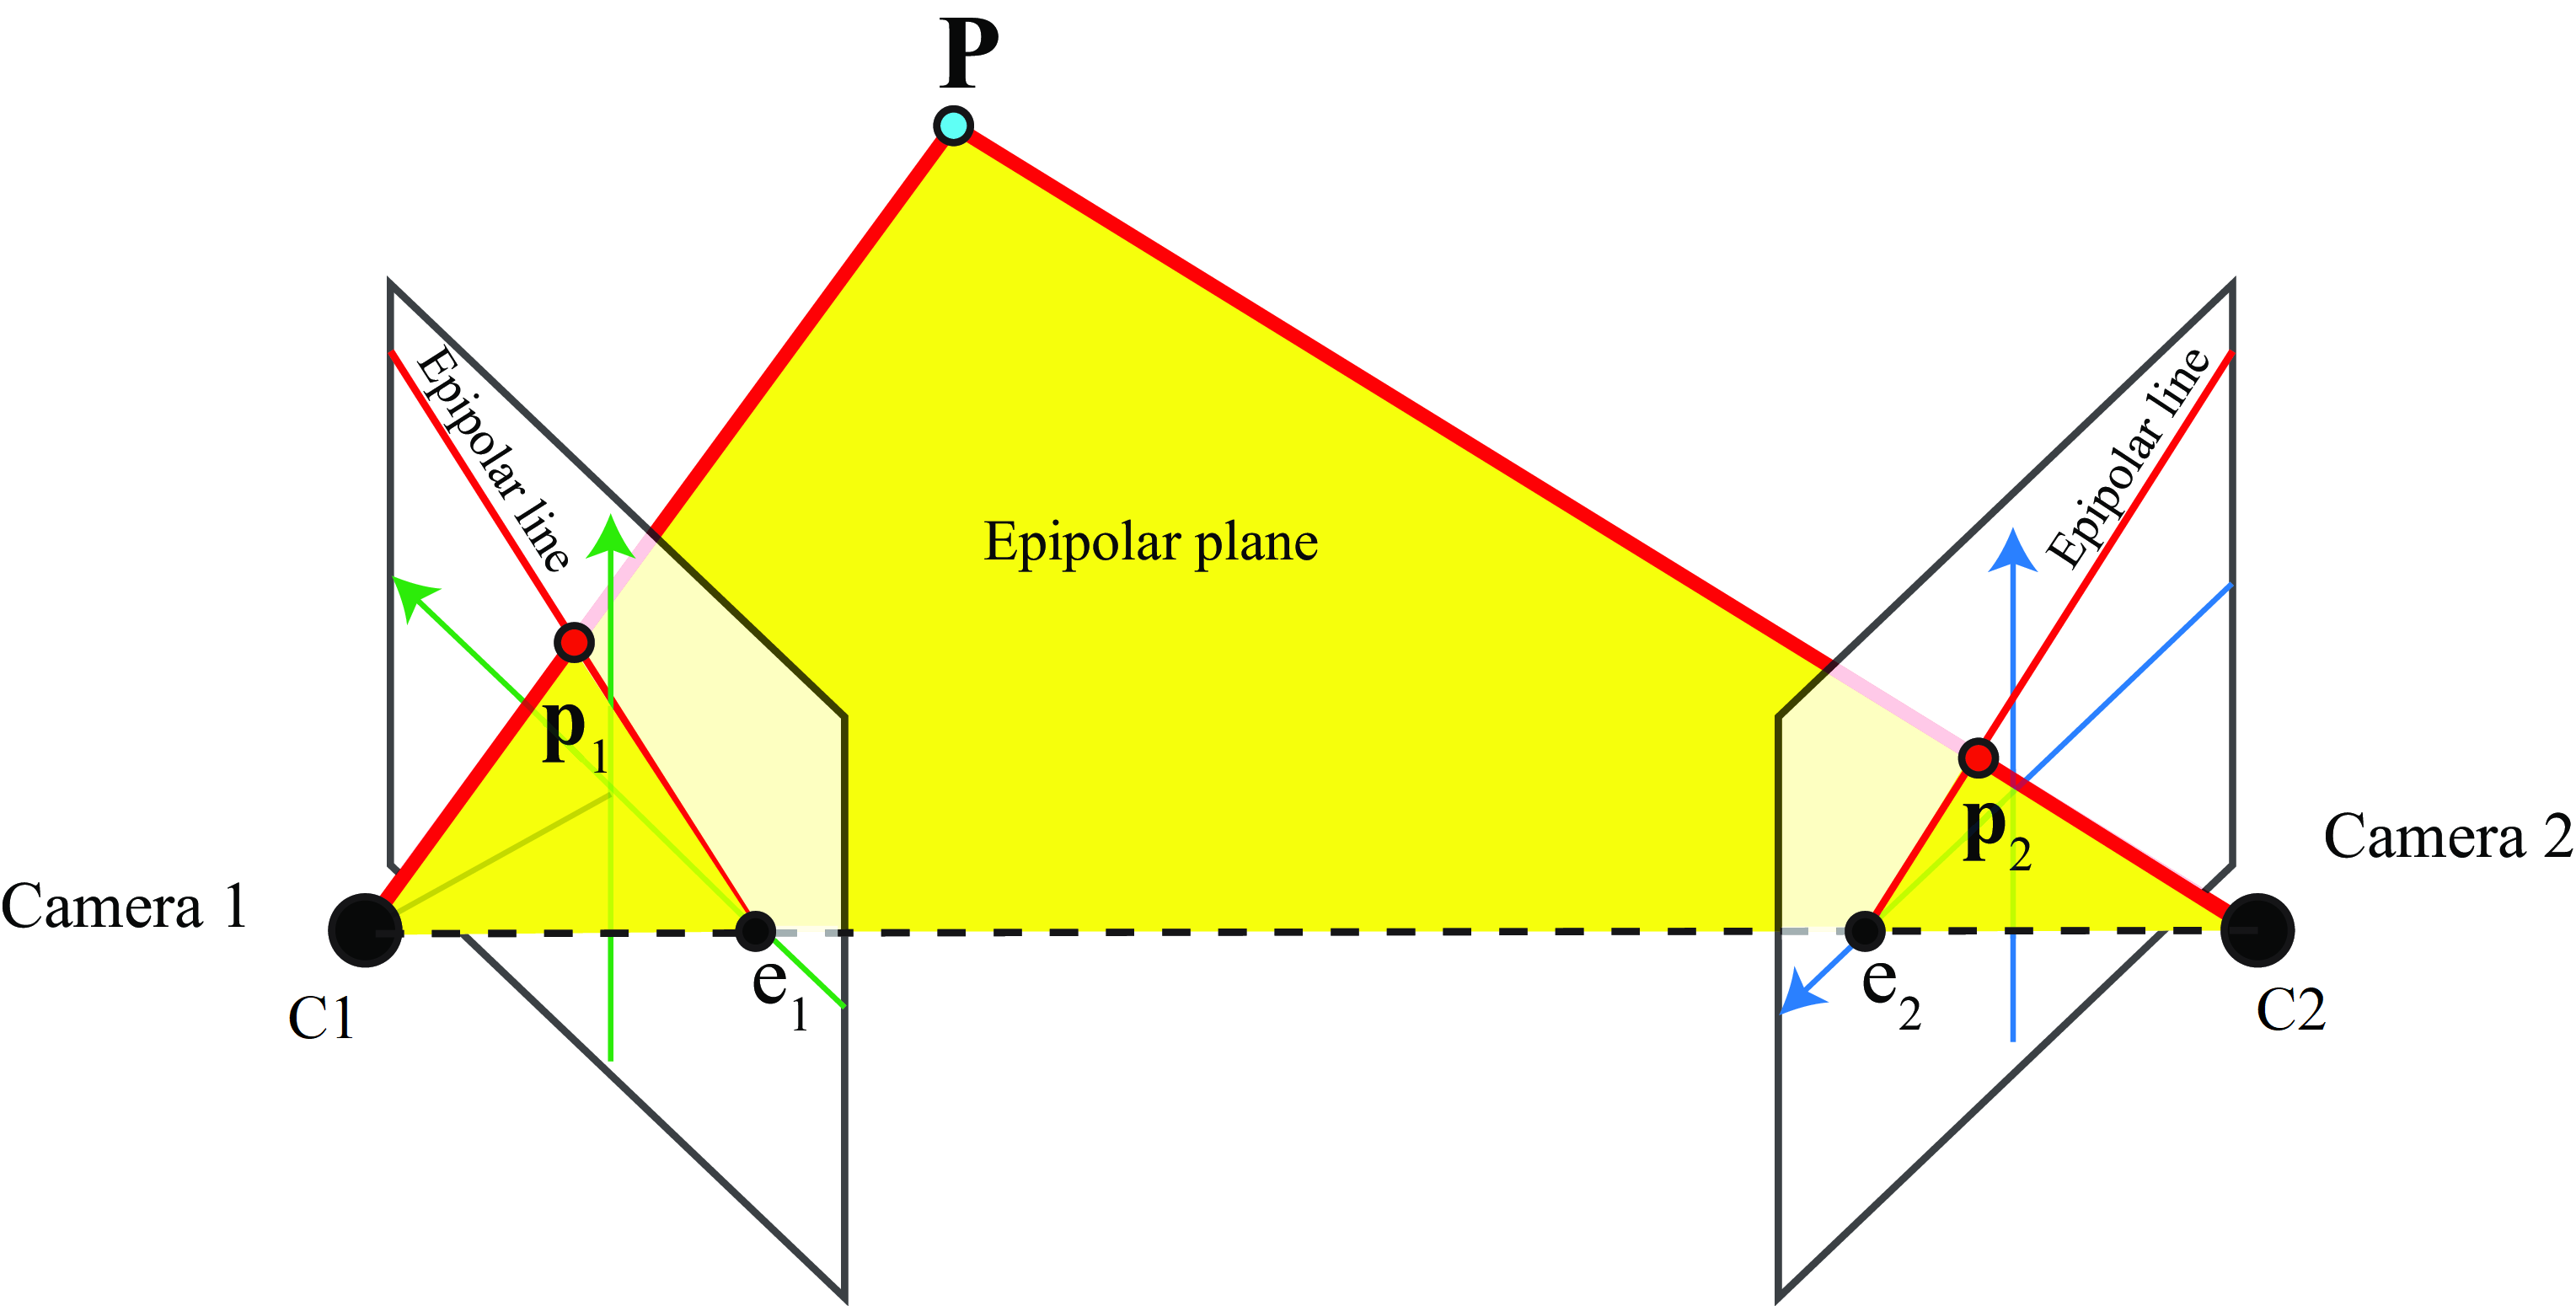
\includegraphics[width=1\linewidth]{epipolar_geometry.png}
    \caption{El diagrama de un estudio para un punto P.}
    \label{fig:diagrama_epipolar}
\end{figure}

A partir de esta configuración espacial, se definen los elementos analíticos fundamentales:

\begin{definition}[Plano epipolar]
Geométricamente, el punto tridimensional $\mathbf{X}$ y los centros ópticos $\mathbf{C}_1$ y $\mathbf{C}_2$ de ambas cámaras determinan un plano en el espacio, que denominaremos \textit{plano epipolar} $\pi$.
\end{definition}

\vspace{2ex}

Las rectas (rayos ópticos) que unen cada centro óptico con el punto $\mathbf{X}$ intersecan los planos imagen exactamente en los puntos de correspondencia $\mathbf{x}_1$ y $\mathbf{x}_2$.

\begin{definition}[Línea base y Epípolos]
    La recta que une de forma directa ambos centros ópticos, $\overline{\mathbf{C}_1 \mathbf{C}_2}$, recibe el nombre de \textit{línea base}. Se denominan \textit{epípolos} a los puntos de intersección de esta recta con los planos imagen, denotados como $\mathbf{e}_1$ y $\mathbf{e}_2$. 
\end{definition}

\vspace{2ex}

Algebraicamente, se puede calcular el epípolo como la proyección del centro óptico de una cámara en el plano de la otra:
\[
    \mathbf{e}_1 = P_1 \mathbf{C}_2, \quad \mathbf{e}_2 = P_2 \mathbf{C}_1
\]

\begin{definition}[Líneas epipolares]
    Llamaremos \textit{líneas epipolares} a las intersecciones del plano epipolar $\pi$ con los planos imagen de ambas cámaras, denotadas por $\mathbf{l}_1$ y $\mathbf{l}_2$. 
\end{definition}

\vspace{2ex}

\begin{observacion}
    Dado que todos los planos epipolares posibles deben contener a la línea base, el conjunto de puntos de la escena genera un haz de planos epipolares cuyo eje es dicha línea base. Esto se traduce en un haz de líneas epipolares en cada plano imagen que convergen obligatoriamente en sus respectivos epípolos $\mathbf{e}_1$ y $\mathbf{e}_2$.
\end{observacion}

\subsection{La Matriz Fundamental}

La matriz fundamental es la representación algebraica de la geometría epipolar que establece la correspondencia geométrica entre dos vistas. A diferencia de una homografía, no constituye una aplicación punto a punto, sino una correlación proyectiva $F: P\mathbb{R}^2 \longrightarrow P\mathbb{R}^{2*}$, donde $P\mathbb{R}^{2*}$ es el espacio de las rectas del proyectivo $P\mathbb{R}^2$. Esta aplicación asigna a cada punto homogéneo de la primera imagen su recta epipolar correspondiente en el otro plano imagen. Algebraicamente, se representa mediante una matriz de dimensiones $3 \times 3$.

A continuación, se desarrolla la deducción analítica para obtener la expresión explícita de dicha matriz.

\subsubsection{Derivación de la Matriz Fundamental}

La deducción de la matriz fundamental se obtiene construyendo algebraicamente la recta epipolar $\mathbf{l}_2$ a partir del rayo óptico retroproyectado desde la primera cámara.

Para un punto $\mathbf{x}_1$ en la primera imagen, el rayo óptico correspondiente en el espacio tridimensional está constituido por la recta que une el centro óptico $\mathbf{C}_1$ con el conjunto de puntos del espacio que se proyectan en $\mathbf{x}_1$. Un punto particular de este rayo se puede obtener algebraicamente utilizando la pseudoinversa de la matriz de cámara, denotada como $P_1^+$, esto es $P_1^+ \in \mathbf{M}_{3 \times 4}$ tal que, $P_1 P_1^+ = I_{3 \times 3}$. Usando esto, el punto tridimensional $\mathbf{X} = P_1^+ \mathbf{x}_1$ pertenece a dicho rayo, puesto que $P_1 \mathbf{X} = P_1 (P_1^+ \mathbf{x_1}) = \mathbf{x}_1$.

La línea epipolar $\mathbf{l}_2$ en la segunda vista es la proyección geométrica de este rayo óptico bajo la acción de la segunda cámara $P_2$. En el plano dual $\mathbb{P}^{2*}$, una recta queda unívocamente definida por el producto vectorial de dos puntos distintos que pertenezcan a ella. Por tanto, se proyectan los dos puntos tridimensionales conocidos del rayo sobre la segunda imagen:

\begin{enumerate}
    \item La proyección del centro óptico de la primera cámara, $\mathbf{C}_1$, es por definición el segundo epípolo:
    \[
        \mathbf{e}_2 = P_2 \mathbf{C}_1
    \]
    \item La proyección del punto retroproyectado $\mathbf{X}$ proporciona un segundo punto de referencia sobre el plano imagen:
    \[
        \mathbf{x}'_2 = (P_2 P_1^+) \mathbf{x}_1
    \]
\end{enumerate}

La línea epipolar se calcula como la recta homogénea que interseca ambos puntos proyectados mediante el producto vectorial:
\[
    \mathbf{l}_2 = \mathbf{e}_2 \times \mathbf{x}'_2 = [\mathbf{e}_2]_\times (P_2 P_1^+ \mathbf{x}_1)
\]
donde $[\mathbf{e}_2]_\times$ representa la matriz antisimétrica de rango 2 asociada al vector del epípolo. 

Por asociatividad del producto matricial, la ecuación se reescribe como:
\[
    \mathbf{l}_2 = \left( [\mathbf{e}_2]_\times P_2 P_1^+ \right) \mathbf{x}_1
\]

De aquí, se deduce la expresión analítica explícita general para la Matriz Fundamental:
\begin{equation}
    F = [\mathbf{e}_2]_\times P_2 P_1^+
\end{equation}

\subsubsection{La restricción epipolar y propiedades de la matriz fundamental}

Finalmente, la restricción de incidencia que estipula que el punto homólogo real $\mathbf{x}_2$ debe yacer sobre su línea epipolar ($\mathbf{x}_2^T \mathbf{l}_2 = 0$) conduce a la ecuación fundamental de la geometría de dos vistas:
\begin{equation}
    \mathbf{x}_2^{T} F \mathbf{x}_1 = 0
\end{equation}

Esto se debe cumplir ya que, si $\mathbf{x}_1$ corresponde con $\mathbf{x}_2$, entonces, $\mathbf{x_2} \in F \mathbf{x_1} = l_2 \Longrightarrow  \mathbf{x_2}^T l_2 =  \mathbf{x_2}^t F  \mathbf{x_1} = 0$ . Esto significa que los puntos de los centros ópticos $\mathbf{C}_1, \mathbf{C}_2$ y las proyecciones $\mathbf{x}_1, \mathbf{x}_2$ de un punto tridimensional deben ser coplanarios.

Esta relación es la base analítica de la geometría de dos vistas. Las propiedades fundamentales de la matriz $F$ son las siguientes:

\begin{itemize}
    \item \textbf{Rango y singularidad:} $F$ es una matriz homogénea de tamaño $3 \times 3$ con rango estricto 2, lo que implica que $\det(F) = 0$.
    \item \textbf{Transposición:} Si $F$ es la matriz fundamental del par de cámaras $(P_1, P_2)$, entonces $F^{T}$ es la matriz fundamental del par inverso $(P_2, P_1)$.
    \item \textbf{Correlación epipolar:} Para cualquier punto $\mathbf{x}_1$ en la primera imagen, su línea epipolar correspondiente en la segunda es $\mathbf{l}_2 = F \mathbf{x}_1$. Inversamente, $\mathbf{l}_1 = F^{T} \mathbf{x}_2$.
    \item \textbf{Espacios nulos (Epípolos):} Como el epípolo $\mathbf{e}_2$ pertenece a todas las líneas epipolares de la segunda imagen, satisface $\mathbf{e}_2^{T} \mathbf{l}_2 = 0$ para todo $\mathbf{x}_1$. Por consiguiente, los epípolos conforman los espacios nulos a izquierda y derecha de la matriz: $\mathbf{e}_2^{T} F = \mathbf{0}$ y $F \mathbf{e}_1 = \mathbf{0}$.
\end{itemize}

Respecto a su parametrización, una matriz de $3 \times 3$ posee 9 elementos. Al estar definida salvo un factor de escala, es una matriz homogénea, sus grados de libertad se reducen a 8. La restricción adicional de singularidad, es decir $\det(F)=0$, deja a la matriz fundamental con \textbf{7 grados de libertad}. Geométricamente, esto equivale a los 4 grados de libertad de ambos epípolos sumados a los 3 grados de la transformación proyectiva 1D que relaciona los haces de rectas epipolares.

\subsubsection{Estructura de la Matriz Fundamental}
La matriz fundamental se puede descomponer analíticamente en el producto de una matriz antisimétrica y una homografía general:

\[
    F = [\mathbf{e}_2]_\times H
\]
Donde $[\mathbf{e}_2]_\times$ representa la representación matricial del producto vectorial por el segundo epípolo y $H$ es una homografía proyectiva. Dado que la matriz antisimétrica tiene rango 2 y la homografía rango 3, el producto preserva la singularidad estipulada:

\[
    \text{rango}(F) = \text{rango}([\mathbf{e}_2]_\times H) = 2
\]

Si se emplea la pseudoinversa de la primera cámara ($P_1^+$) para retroproyectar el rayo óptico y transferirlo a la segunda vista, la homografía interna toma la forma $H = P_2 P_1^{+}$. Sustituyendo este resultado, se obtiene la formulación explícita general:

\[
    F = [\mathbf{e}_2]_\times P_2 P_1^{+}
\]

\subsubsection{Cálculo de la Matriz Fundamental}
Existen múltiples métodos para estimar $F$ a partir de correspondencias de puntos bidimensionales. Se exponen a continuación los dos enfoques lineales clásicos.

\paragraph{El Algoritmo de los 8 Puntos Normalizado}~\\
Este algoritmo estima la matriz $F$ resolviendo un sistema lineal sobredeterminado a partir de $n \ge 8$ correspondencias de puntos $(\mathbf{x}_i, \mathbf{x}'_i)$.

\begin{enumerate}
    \item \textbf{Normalización (Hartley):} Se aplican transformaciones afines $T$ y $T'$ a las coordenadas de la imagen para trasladar el centroide de los puntos al origen $(0,0)^T$ y escalar su distancia media al origen a $\sqrt{2}$. Las coordenadas normalizadas son $\hat{\mathbf{x}}_i=T \mathbf{x}_i$ y $\hat{\mathbf{x}}'_i=T' \mathbf{x}'_i$.
    \item \textbf{Solución lineal:} Cada par genera una ecuación $\hat{\mathbf{x}}'^T_i \hat{F} \hat{\mathbf{x}}_i = 0$. Apilando las ecuaciones se forma un sistema $A \mathbf{f} = \mathbf{0}$, donde $\mathbf{f}$ contiene los elementos de $\hat{F}$. La solución se obtiene calculando el vector propio asociado al menor valor singular de $A$ mediante la Descomposición en Valores Singulares (SVD).
    \begin{figure}[H]
    \centering
    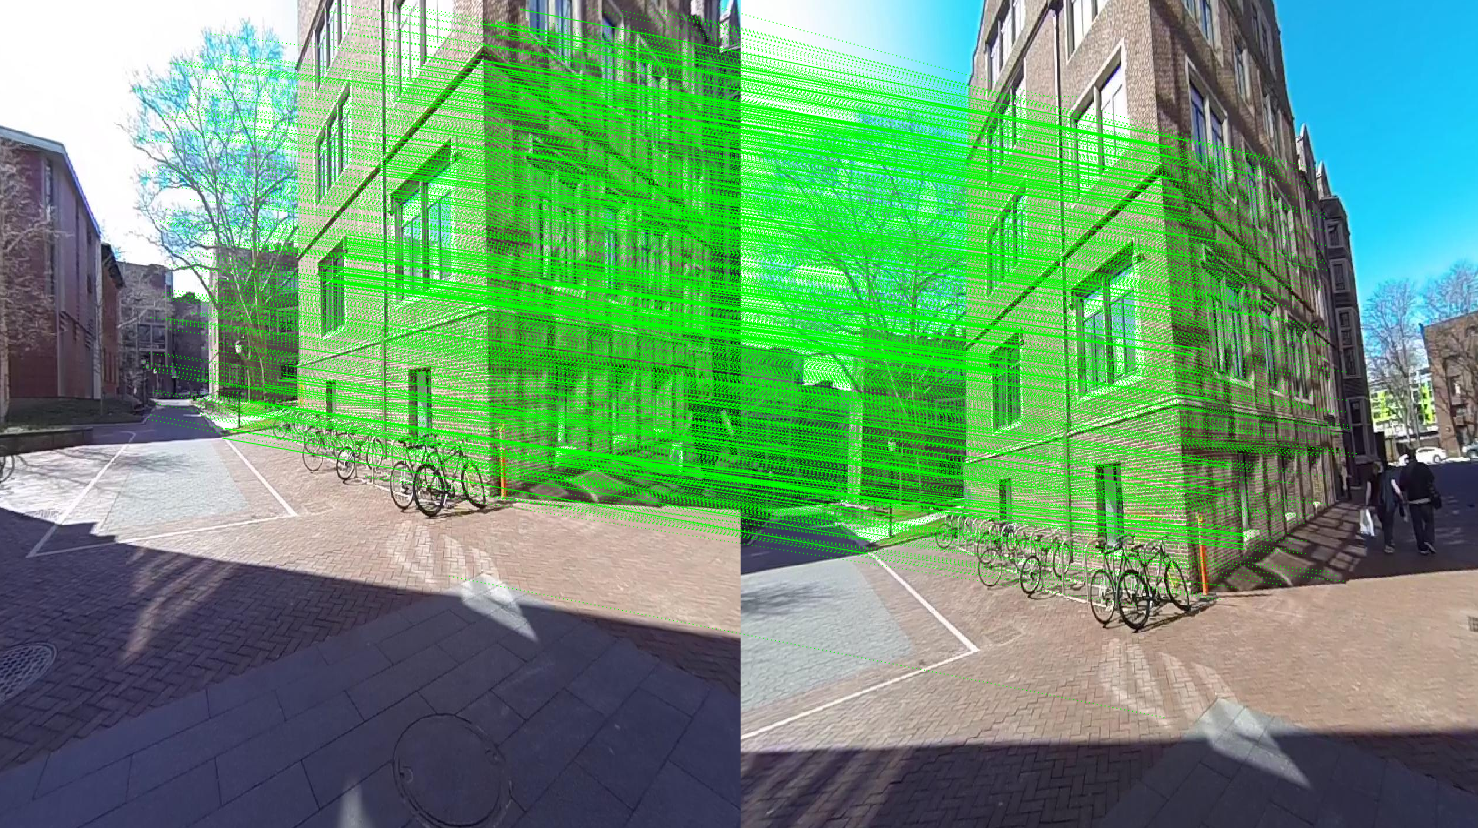
\includegraphics[width=0.9\linewidth]{problemaError.png}
    \caption{En esta figura se observan las correspondecias de puntos de dos imágenes de una escena. Las rectas verdes al no ser paralelas reflejan que debido al ruido y errores de localización de los puntos de interés, ninguna solución satisface todas las ecuaciones a la vez. Esto motiva el uso de SVD.}
    \label{fig:errores}
\end{figure}
    \item \textbf{Imposición de rango 2:} Se descompone la matriz resultante $\hat{F}$ mediante SVD, se anula su menor valor singular y se recompone para obtener una matriz $\hat{F}'$ estrictamente singular.
    \item \textbf{Desnormalización:} Finalmente, la matriz se proyecta de vuelta al espacio de coordenadas original:
    \begin{equation}
        F = T'^{T} \hat{F}' T
    \end{equation}
\end{enumerate}

\paragraph{El Algoritmo de los 7 Puntos}~\\
Aprovechando que $F$ posee 7 grados de libertad, es posible resolver el sistema utilizando un conjunto mínimo de 7 correspondencias.
En este caso, el sistema lineal homogéneo $A \mathbf{f} = \mathbf{0}$ posee un espacio nulo de dimensión 2. Por tanto, la matriz se expresa como una combinación lineal de las dos matrices base:
\begin{equation}
    F = \alpha F_1 + (1-\alpha)F_2
\end{equation}
Al imponer la restricción de singularidad $\det(F) = 0$, se genera un polinomio cúbico en $\alpha$, el cual proporciona 1 o 3 soluciones reales. Se selecciona la matriz que minimice el error geométrico sobre el conjunto completo de datos.

\subsubsection{Estimación Robusta mediante RANSAC}
En un escenario real, las correspondencias automáticas contienen valores atípicos (outliers). Para estimar $F$ de forma robusta, se integra el algoritmo de 7 u 8 puntos dentro del bucle probabilístico RANSAC:

\begin{enumerate}
    \item \textbf{Extracción y Emparejamiento:} Se detectan puntos de interés (keypoints) en ambas imágenes y se establecen correspondencias tentativas basadas en descriptores locales.
    \begin{figure}[H]
        \centering
        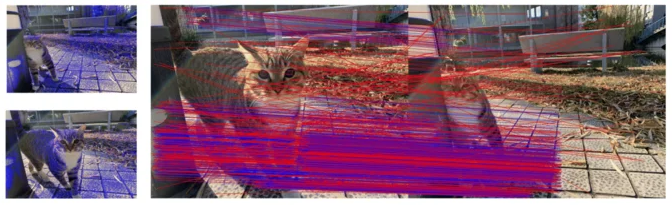
\includegraphics[width=0.75\linewidth]{ransac aux2.png}
        \caption{Correspondencias tentativas entre dos vistas de la misma escena. Las líneas conectan puntos de interés con descriptores similares. El patrón caótico de líneas se debe a la presencia de \textit{inliers} y \textit{outliers}, al aplicar RANSAC se filtran los \textit{outliers}, conservando únicamente los \textit{inliers}.}
        \label{fig:ransac_correspondencias}
    \end{figure}
    \item \textbf{Muestreo iterativo:} Durante $N$ iteraciones:
    \begin{enumerate}
        \item Se selecciona aleatoriamente un subconjunto mínimo (ej. 7 u 8 correspondencias) para instanciar una matriz candidata $F_k$.
        \item Se evalúa el consenso general computando el error de todos los pares frente a $F_k$ (generalmente la distancia de Sampson o la distancia epipolar ortogonal $d_\perp$).
        \item Se contabiliza el número de \textit{inliers} (correspondencias con error inferior a un umbral $\tau$).
    \end{enumerate}
    \begin{figure}[H]
        \centering
        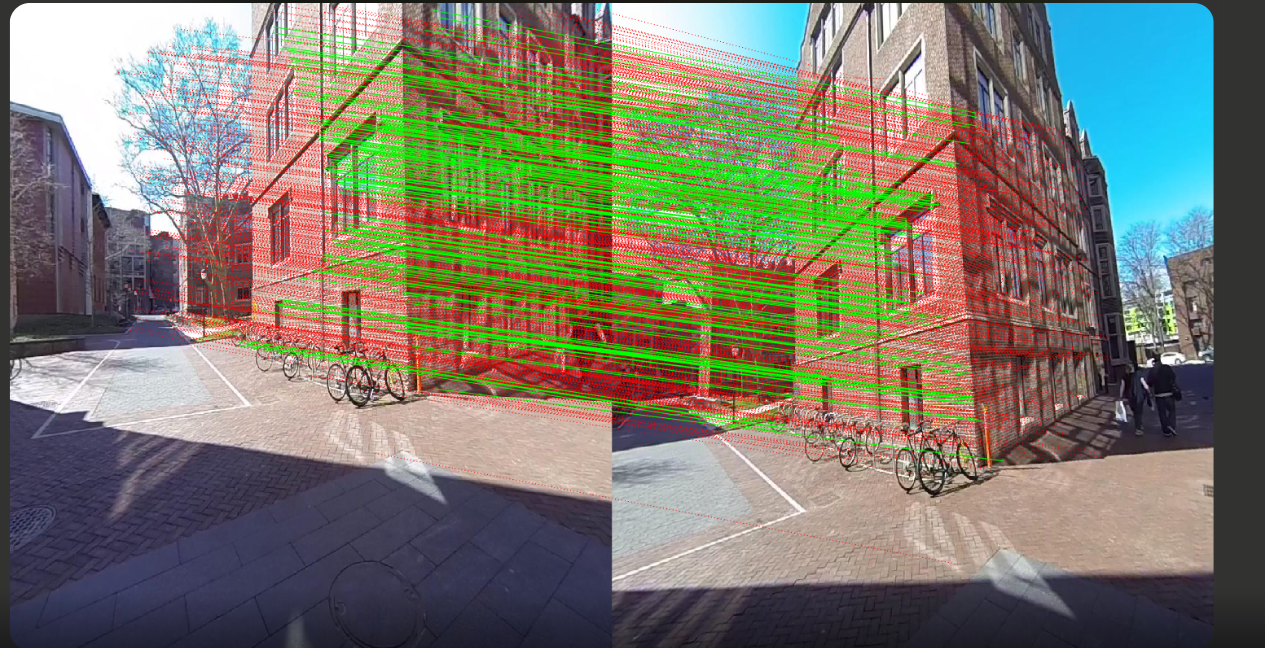
\includegraphics[width=0.75\linewidth]{ransac aux3.png}
        \caption{Resultado de aplicar RANSAC sobre las correspondencias tentativas. En verde se muestran los  \textit{inliers} que el algoritmo ha identificado como coherentes con la matriz $\mathbf{F}$ estimada, y en rojo los  \textit{outliers} descartados por ser inconsistentes con el modelo.}
        \label{fig:ransac}
    \end{figure}
    \item \textbf{Reestimación final:} Se retiene la matriz $F$ que maximice el soporte (mayor número de \textit{inliers}). Finalmente, se recalcula $F$ aplicando el algoritmo de 8 puntos normalizado utilizando exclusivamente todo el conjunto de \textit{inliers} validados.
\end{enumerate}

\subsection{Matriz Esencial}






%----------------------------------------------------------------------------------------
%	RESULTS AND DISCUSSION
%----------------------------------------------------------------------------------------

\section{Conclusión}


%----------------------------------------------------------------------------------------
%	BIBLIOGRAPHY
%----------------------------------------------------------------------------------------

\renewcommand{\refname}{\spacedlowsmallcaps{References}} % For modifying the bibliography heading

\bibliographystyle{unsrt}

\bibliography{sample.bib} % The file containing the bibliography

%----------------------------------------------------------------------------------------

\end{document}
